\documentclass[sigplan,10pt]{acmart}

\AtBeginDocument{%
  \providecommand\BibTeX{{%
    \normalfont B\kern-0.5em{\scshape i\kern-0.25em b}\kern-0.8em\TeX}}}

\usepackage{subcaption}
\usepackage{tikz}
\usepackage{fancyvrb}
\usepackage{xcolor}
\usepackage{breqn}

\usetikzlibrary{decorations.pathmorphing}
\tikzstyle{vertex} = [circle, minimum width=10pt,draw,inner sep=0pt]
\tikzstyle{vertex2} = [circle, minimum width=40pt,draw,inner sep=0pt]
\tikzstyle{server} = [rectangle, rounded corners,minimum width=2cm,minimum height=2.5cm,draw=black]
\tikzstyle{local} = [thick,->,>=stealth]
\tikzstyle{dist} = [thick,dashed,->,>=stealth]
\tikzstyle{node}=[circle,draw,radius=0.3, align=center]

\definecolor{grey}{rgb}{0.52, 0.52, 0.51}
\definecolor{red}{rgb}{0.7, 0.11, 0.11}
\definecolor{blue}{rgb}{0.0, 0.0, 0.55}
\definecolor{green}{rgb}{0.0, 0.42, 0.24}

%% Rights management information.  This information is sent to you
%% when you complete the rights form.  These commands have SAMPLE
%% values in them; it is your responsibility as an author to replace
%% the commands and values with those provided to you when you
%% complete the rights form.
\setcopyright{acmcopyright}
\copyrightyear{2020}
\acmYear{2020}
\acmDOI{10.1145/1122445.1122456}

%% These commands are for a PROCEEDINGS abstract or paper.
\acmConference[PaPoC '20]{PaPoC '20: Proceedings of the 7th Workshop on Principles and Practice of Consistency for Distributed Data}{April 27, 2020}{Heraklion, Crete, Greece}
\acmBooktitle{PaPoC '20: Proceedings of the 7th Workshop on Principles and Practice of Consistency for Distributed Data, April 27, 2020, Heraklion, Crete, Greece}
\acmPrice{15.00}
% \acmISBN{978-1-4503-XXXX-X/18/06}


%%
%% Submission ID.
%% Use this when submitting an article to a sponsored event. You'll
%% receive a unique submission ID from the organizers
%% of the event, and this ID should be used as the parameter to this command.
%%\acmSubmissionID{123-A56-BU3}

%%
%% The majority of ACM publications use numbered citations and
%% references.  The command \citestyle{authoryear} switches to the
%% "author year" style.
%%
%% If you are preparing content for an event
%% sponsored by ACM SIGGRAPH, you must use the "author year" style of
%% citations and references.
%% Uncommenting
%% the next command will enable that style.
%%\citestyle{acmauthoryear}

%%
%% end of the preamble, start of the body of the document source.
\begin{document}

%%
%% The "title" command has an optional parameter,
%% allowing the author to define a "short title" to be used in page headers.
\title{Preserving Reciprocal Consistency in Distributed Graph Databases}

%%
%% The "author" command and its associated commands are used to define
%% the authors and their affiliations.
%% Of note is the shared affiliation of the first two authors, and the
%% "authornote" and "authornotemark" commands
%% used to denote shared contribution to the research.
\author{Jack Waudby}
\email{j.waudby2@ncl.ac.uk}
\affiliation{%
  \institution{Newcastle University}
  \city{Newcastle}
  \country{UK}
  \postcode{NE4 5TG}
}

\author{Paul Ezhilchelvan}
\email{paul.ezhilchelvan@ncl.ac.uk}
\orcid{0000-0002-6190-5685}
\affiliation{%
  \institution{Newcastle University}
  \city{Newcastle}
  \country{UK}
  \postcode{NE4 5TG}
}

\author{Jim Webber}
\email{jim.webber@neo4j.com}
\affiliation{%
  \institution{Neo4j}
  \streetaddress{Union House,182-194 Union Street}
  \city{London}
  \country{UK}
  \postcode{SE1 0LH}}

\author{Isi Mitrani}
\email{isi.mitrani@ncl.ac.uk}
\orcid{0000-0002-7797-7755}
\affiliation{%
  \institution{Newcastle University}
  \city{Newcastle}
  \country{UK}
  \postcode{NE4 5TG}
}

\renewcommand{\shortauthors}{Ezhilchelvan, et al.}

\begin{abstract}
% In this paper the notion of \textit{reciprocal consistency}, a important constraint specific to graph databases, is formalized. If reciprocal consistency is not ensured during transaction processing, a distributed graph database can become operationally corrupt within a short time period relative to database lifetime. Reciprocal consistency can be maintained as a part of enforcing any of several known strong isolation guarantees (e.g., Snapshot Isolation) incurring well established performance costs.

In our earlier work, we identified \emph{reciprocal consistency} as an important constraint specific to graph databases. If it can be lost even with a negligible small probability, subsequent inconsistent reads followed by writes can corrupt a distributed graph database within a time period extremely short relative to database lifetime. Reciprocal consistency can of course be maintained as a part of enforcing any known isolation guarantee incurring well established performance costs. However, in practice distributed graph databases are often built atop BASE databases with few or no isolation guarantees, profiting from increased performance but leaving them susceptible to rapid corruption. A lightweight protocol ensuring reciprocal consistency is presented, catering for application programmers that are interested in maintaining performance and the structural integrity of their distributed graph database. Protocol performance is evaluated through simulations.
\end{abstract}

% \begin{CCSXML}
% <ccs2012>
%  <concept>
%   <concept_id>10010520.10010553.10010562</concept_id>
%   <concept_desc>Computer systems organization~Embedded systems</concept_desc>
%   <concept_significance>500</concept_significance>
%  </concept>
%  <concept>
%   <concept_id>10010520.10010575.10010755</concept_id>
%   <concept_desc>Computer systems organization~Redundancy</concept_desc>
%   <concept_significance>300</concept_significance>
%  </concept>
%  <concept>
%   <concept_id>10010520.10010553.10010554</concept_id>
%   <concept_desc>Computer systems organization~Robotics</concept_desc>
%   <concept_significance>100</concept_significance>
%  </concept>
%  <concept>
%   <concept_id>10003033.10003083.10003095</concept_id>
%   <concept_desc>Networks~Network reliability</concept_desc>
%   <concept_significance>100</concept_significance>
%  </concept>
% </ccs2012>
% \end{CCSXML}

\ccsdesc[500]{Data Management~Graph Databases}
\ccsdesc[300]{Data Management~Reciprocal Consistency}

% \ccsdesc[500]{Computer systems organization~Embedded systems}
% \ccsdesc[300]{Computer systems organization~Redundancy}
% \ccsdesc{Computer systems organization~Robotics}
% \ccsdesc[100]{Networks~Network reliability}

\keywords{Graph Databases, Reciprocal Consistency}


\maketitle

\section{Introduction}
\label{sec:introduction}

Recent years have seen a proliferation in the use of graph processing technologies \cite{Besta2019}. Application areas are wide reaching from healthcare, to social networks and fraud detection \cite{Eifrem2016}. Graph databases model data as a \textit{property graph} \cite{Robinson2015}, vertices represent entities and edges represent the relationships between entities. In addition, properties can be stored on both vertices and edges.

In the storage layer, edges are represented by two reciprocal pointers, one stored with each vertex the edge connects. This allows for bi-directional traversal and improved query performance. An edge is said to be \emph{reciprocally consistent}, if its two end pointers are mutually reciprocal of each other (Details in Section \ref{sec:recipr-cons}).

In practice graphs can be extremely large, sometimes in the magnitude of 100 billion edges \cite{Sahu2017}, exceeding the storage capacity of a single-node database and motivating the need for distributed graph databases. A common design pattern is to partition graph data over several machines in a cluster and use a BASE database \cite{Pritchett2008} for storage, adapted with a graph processing layer (\cite{janusgraph}, \cite{TitanDB}). A caveat with this approach is BASE databases in practice eschew transactional guarantees in order to achieve higher performance.

Recent work \cite{Ezhilchelvan2018} and \cite{Webber2019} highlighted how reciprocal consistency can easily be violated in such a design introducing corruption into the database. Moreover, due to the \emph{Scale-Free} \cite{ScaleFree} property exhibited by many real world graphs, this corruption can propagate through the database at alarmingly rates.

Preserving reciprocal consistency requires some degree of coordination between partitions in the presence of concurrent modifications. This paper proposes and analyses a light-weight protocol that ensures reciprocal consistency in operational contexts where concurrency control mechanisms are done away with for sake of performance.

%The contribution of this paper is the description of a protocol that ensures reciprocal consistency, preserving structural integrity in a distributed graph database in a transaction processing setting. The protocol maintains this guarantee provided certain condition hold. If these conditions are violated corruption can still occur. The protocol's impact on the rate of database corruption and its performance is evaluated and discussed.

%The key finding is whilst the protocol reduces the chance of initial corruption of clean database records, due to the scale-free topology corruption propagates alarmingly quick even for modest transaction arrival rates. This motivates the use of deterministic reciprocal consistency protocols or the use of protocols with stronger isolation guarantees, which subsume reciprocal consistency (\cite{Bailis2014}, \cite{Berenson1995}, \cite{Bernstein1987}).

\section{Reciprocal Consistency}
\label{sec:recipr-cons}

In the property graph data model edges have direction, each edge having a pair of \emph{source} and \emph{destination} vertices. In the storage layer, edge information is stored with \textbf{both} the source and destination vertices. This facilitates bi-directional edge traversal and allows for better query performance.

A common approach to storing graphs (arising from JanusGraph \cite{janusgraph} and TitanDB \cite{TitanDB}) is for database records to represent vertices containing both data values and an adjacency list containing edge \emph{pointers} to other vertices, Figure \ref{adj-list}. In this representation an edge has \emph{reciprocal} entries in the adjacency lists of the vertices the edge connects. A query reading either the source or destination vertex should be able to reify the edge correctly, returning consistent results. When the adjacency list entries for a given edge are mutually compatible like this, that edge is said to be \emph{reciprocally consistent}, a form of referential integrity.

\begin{figure}[ht]
  \centering
  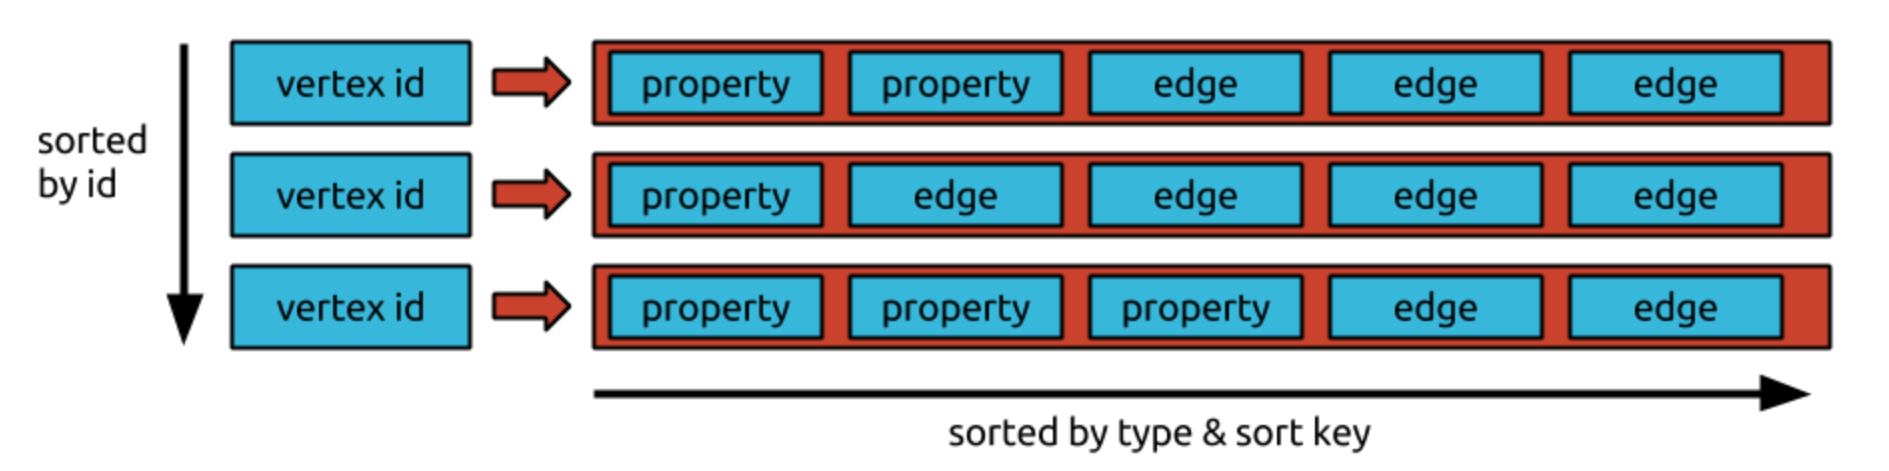
\includegraphics[width=\linewidth]{./images/janusgraph-adj-list}
  \caption{Database records representing vertices, containing data values and adjacency lists \cite{janusgraph}.}
  \label{adj-list}
\end{figure}

Consider, for example, the statement that Tolkien \textit{wrote} The Hobbit. It is expressed using vertices \emph{a} and \emph{b}, for Tolkien and The Hobbit respectively, and an edge \textit{wrote} running from \emph{a} (source) to \emph{b} (destination).

Using openCypher \cite{openCypher} this can be represented by:
\begin{Verbatim}[commandchars=\\\{\},fontsize=\small,xleftmargin=.2in]
\textcolor{blue}{MATCH} (a:\textcolor{green}{Person}), (b:\textcolor{green}{Book})
\textcolor{blue}{WHERE} a.\textcolor{red}{name} = 'Tolkien' \textcolor{blue}{AND} b.\textcolor{red}{title} = 'The Hobbit'
\textcolor{blue}{CREATE} (a)-[w:\textcolor{green}{WROTE}]->(b)
\end{Verbatim}

Adjacency lists of both \emph{a} and \emph{b} record information about the edge and this information is mutually reciprocal (or inverse) of each other: \emph{a}'s list will indicate `\emph{a} \emph{wrote} \emph{b}' while \emph{b}'s will have `\emph{b} \emph{written} by \emph{a}'. Thus, a query `list all titles by the author who wrote The Hobbit' can be answered starting at (destination vertex) \emph{b} and then traversing to (source vertex) \emph{a}, even though the edge is ``directed'' from \emph{a} to \emph{b} at model level abstraction.

\section{Distributed Graph Databases}

A distributed graph database employs a shared-nothing architecture, partitioning a graph between a number of loosely cooperating servers. Graph partitioning is non-trivial and a common approach is to use a $k$-balanced edge cut \cite{Huang2016}. The objective of such an approach is to minimize the proportion of edges that span partitions in a manner that balances the distribution of vertices to partitions. Intra-partition edges are referred to as \textit{local edges} and inter-partition edges are referred to as \textit{distributed edges}, Figure \ref{dist-graph}. The proportion of distributed edges is always non-negligible ranging from 25-75\% \cite{Huang2016}.

\begin{figure}[ht]
  \centering
    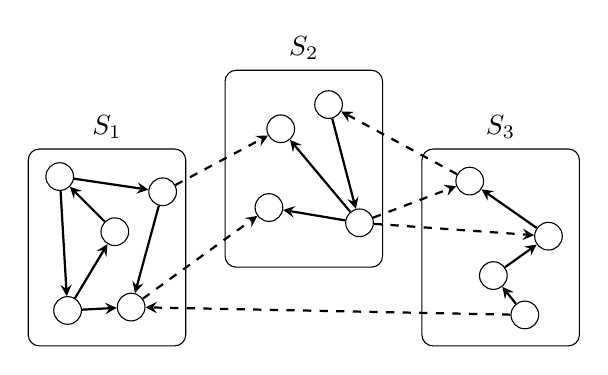
\begin{tikzpicture}[node distance=1cm]

    \node (s1) [server,label=$S_1$] {};
    \node (s2) [server, right of=s1,xshift=1.5cm,yshift=1cm,label=$S_2$] {};
    \node (s3) [server, right of=s1,xshift=4cm,label=$S_3$] {};

    \node (v1) [vertex,xshift=-0.5cm,yshift=-0.8cm] {};
    \node (v2) [vertex, above of=v1,xshift=-0.1cm,yshift=0.7cm] {};
    \node (v3) [vertex, above of=v1,xshift=0.6cm] {};
    \node (v4) [vertex, below right of=v3,xshift=-0.5cm,yshift=-0.25cm] {};
    \node (v5) [vertex, above right of=v3,xshift=-0.1cm,yshift=-0.2cm] {};
    \node (v6) [vertex, right of=v5,xshift=0.5cm,yshift=0.8cm] {};
    \node (v7) [vertex, below of=v6, xshift=-0.15cm,yshift=0cm] {};
    \node (v8) [vertex, right of=v4, yshift=-0.1cm,xshift=4cm] {};
    \node (v9) [vertex, above of=v8,xshift=-0.4cm,yshift=-0.5cm] {};
    \node (v10) [vertex, above of=v9,xshift=-1.7cm,yshift=-0.33cm] {};
    \node (v11) [vertex, right of=v9,yshift=0.5cm,xshift=-0.3cm] {};
    \node (v12) [vertex, above of=v11,yshift=-0.3cm,xshift=-1cm] {};
    \node (v13) [vertex, above right of=v6,yshift=-0.4cm,xshift=-0.1cm] {};
    \draw [local] (v2) -- (v1);
    \draw [local] (v1) -- (v3);
    \draw [local] (v3) -- (v2);
    \draw [local] (v2) -- (v5);
    \draw [local] (v1) -- (v4);
    \draw [local] (v5) -- (v4);
    \draw [dist] (v5) -- (v6);
    \draw [dist] (v4) -- (v7);
    \draw [dist] (v8) -- (v4);
    \draw [local] (v8) -- (v9);
    \draw [local] (v9) -- (v11);
    \draw [local] (v10) -- (v7);
    \draw [dist] (v10) -- (v12);
    \draw [dist] (v12) -- (v13);
    \draw [local] (v10) -- (v6);
    \draw [dist] (v10) -- (v11);
    \draw [local] (v13) -- (v10);
    \draw [local] (v11) -- (v12);
    \end{tikzpicture}
  \caption{A graph partitioned across $k=3$ servers in a cluster. Dashed lines represent distributed edges and solid lines represent local edges.}
  \Description{Graph representation.}
  \label{dist-graph}
\end{figure}

Adjacency lists can now contain edge pointers to vertices on remote servers. Maintaining reciprocal consistency for such distributed edges is challenging - especially given a common architecture employed by contemporary distributed graph databases. Often they use an existing BASE database to store data, which has been adapted with a programmatic API or query language expressed in terms of edges and vertices along with some gluecode to bind that interface to the underlying database. Superficially, opting for this design appears to be a good choice: the user has the modeling convenience of graphs with the operational characteristics from the underlying database. However, the problem with this design is the (lack of) transactional semantics are inherited from the underlying store. Using the primitives provided by BASE databases maintaining reciprocal consistency for local edges is straightforward, this is not true for distributed edges. The lack of concurrency control across partitions means it is possible that concurrent updates can interleave in a manner that violates reciprocal consistency.


\section{Corruption in BASE  Distributed Graph Databases}
\label{sec:db-corruption}

\begin{figure*}[ht]
  \centering
  \begin{subfigure}[b]{0.3\textwidth}
    \centering
    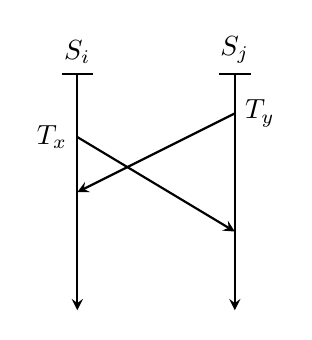
\begin{tikzpicture}
      \draw [thick] (1.3,3) -- (1.7,3);
      \draw [thick,<-,>=stealth] (1.5,0) -- (1.5,3) node[anchor=south] {$S_i$};
      \draw [thick] (3.3,3) -- (3.7,3);
      \draw [thick,<-,>=stealth] (3.5,0) -- (3.5,3) node[anchor=south] {$S_j$};
      \draw [thick,<-,>=stealth] (1.5,1.5) -- (3.5,2.5)  node[right] {$T_y$};
      \draw [thick,->,>=stealth] (1.5,2.2) node[left] {$T_x$} -- (3.5,1);
    \end{tikzpicture}
    \caption{}
  \end{subfigure}%
  \begin{subfigure}[b]{0.3\textwidth}
    \centering
    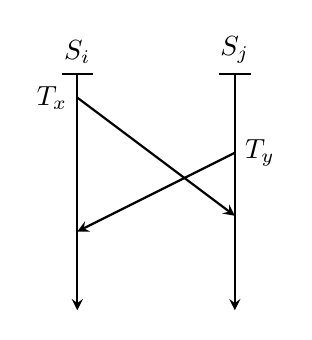
\begin{tikzpicture}
      \draw [thick] (5.3,3) -- (5.7,3);
      \draw [thick,<-,>=stealth] (5.5,0) -- (5.5,3) node[anchor=south] {$S_i$};
      \draw [thick] (7.3,3) -- (7.7,3);
      \draw [thick,<-,>=stealth] (7.5,0) -- (7.5,3) node[anchor=south] {$S_j$};
      \draw [thick,<-,>=stealth] (5.5,1) -- (7.5,2)  node[right] {$T_y$};
      \draw [thick,->,>=stealth] (5.5,2.7) node[left] {$T_x$} -- (7.5,1.2);
    \end{tikzpicture}
    \caption{}
  \end{subfigure}%
  \begin{subfigure}[b]{0.3\textwidth}
    \centering
    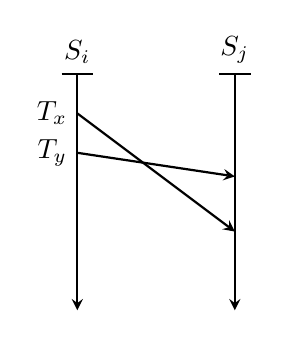
\begin{tikzpicture}
      \draw [thick] (9.3,3) -- (9.7,3);
      \draw [thick,<-,>=stealth] (9.5,0) -- (9.5,3) node[anchor=south] {$S_i$};
      \draw [thick] (11.3,3) -- (11.7,3);
      \draw [thick,<-,>=stealth] (11.5,0) -- (11.5,3) node[anchor=south] {$S_j$};
      \draw [thick,->,>=stealth] (9.5,2.5)  node[left] {$T_x$} -- (11.5,1) ;
      \draw [thick,->,>=stealth] (9.5,2) node[left] {$T_y$} -- (11.5,1.7);
    \end{tikzpicture}
    \caption{}
  \end{subfigure}%
  \caption{Possible interleavings of concurrent transaction's writes to a distributed edge spanning servers $S_i$ and $S_j$ by transactions $T_x$ and $T_y$. In (a) $T_y$ begins writing to the distributed edge before $T_x$, in (b) the converse is true, else they are equivalent. In (c) both transactions begin writing at the same server but overlap in the network and arrive out-of-order.}
  \label{conf-scen}
\end{figure*}

Earlier work investigated how weak isolation across partitions in BASE distributed graph databases can undermine reciprocal consistency of distributed edges, causing irreversible corruption that spreads at alarmingly rates (\cite{Ezhilchelvan2018}, \cite{Webber2019}).

When a given transaction writes a distributed edge it must infact perform two writes, writing reciprocal information at the source and the destination vertices, which say reside on servers $S_i$ and $S_j$ respectively. Concurrent transaction's writes to a distributed edge can interleave producing a distributed edge in a \emph{half-corrupted} state - reciprocal consistency has been violated, Figure \ref{conf-scen}. For such edges there exists a correct and a incorrect entry. Note, the order in which the two writes take place is not constrained. For example, when updating an edge between \emph{a} and \emph{b} it is equally likely to update \emph{a} then \emph{b} as it is to update \emph{b} then \emph{a}. A graph with half-corrupted edges has suffered \emph{structural corruption}.

Now, if subsequent transactions read the incorrect entry of a half-corrupted edge and write further edges, \emph{semantic corruption} has been introduced into the database. Further semantic corruption spreads by the same mechanism. A database is said to be \emph{operationally corrupt} when a significant proportion of its data records are in a semantically corrupted state, rendering the database of little practical use.

To illustrate the process of corruption, consider two transactions $T_x$ and $T_y$. $T_x$ deletes the \emph{wrote} edge and $T_y$ appends a property \emph{year}:
\begin{Verbatim}[commandchars=\\\{\},fontsize=\small,xleftmargin=.2in]
\textcolor{grey}{// Tx}
\textcolor{blue}{MATCH} (a:\textcolor{green}{Person})-[w:\textcolor{green}{WROTE}]->(b:\textcolor{green}{Book})
\textcolor{blue}{WHERE} a.\textcolor{red}{name} = 'Tolkien' \textcolor{blue}{AND} b.\textcolor{red}{title} = 'The Hobbit'
\textcolor{blue}{DELETE} w

\textcolor{grey}{// Ty}
\textcolor{blue}{MATCH} (a:\textcolor{green}{Person})-[w:\textcolor{green}{WROTE}]->(b:\textcolor{green}{Book})
\textcolor{blue}{WHERE} a.\textcolor{red}{name} = 'Tolkien' \textcolor{blue}{AND} b.\textcolor{red}{title} = 'The Hobbit'
\textcolor{blue}{SET} w.\textcolor{red}{year} = 1937
\end{Verbatim}
Any interleaving in Figure \ref{conf-scen} will result in the half-corrupted edge displayed in Figure \ref{half-corrupted}.

\begin{figure}[H]
  \centering
  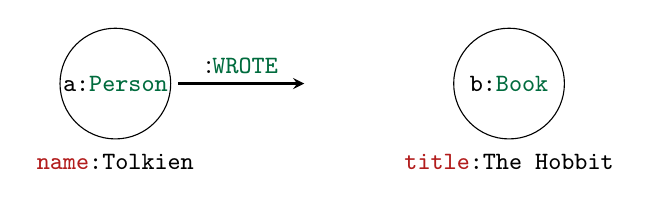
\begin{tikzpicture}[node distance=2cm]
    \node (v1) [vertex2,xshift=0cm,yshift=0cm] {\small{\texttt{a:\textcolor{green}{Person}}}};

    \node (v2) [vertex2,xshift=5cm,yshift=0cm] {\small{\texttt{b:\textcolor{green}{Book}}}};

    \node [below of=v1,yshift=1cm] {\small{\texttt{\textcolor{red}{name}:Tolkien}}};
        \node [below of=v2,yshift=1cm] {\small{\texttt{\textcolor{red}{title}:The Hobbit}}};

    \draw [thick,->,>=stealth] (0.8,0)  -- node [midway,above] {:\textcolor{green}{\small{\texttt{WROTE}}}} (2.4,0);

  \end{tikzpicture}
  \caption{A half-corrupted edge resulting from conflicting transactions.}
  \label{half-corrupted}
\end{figure}

Assume, the correct ordering of transactions is $T_y$ then $T_x$ and the edge between \emph{a} and \emph{b} should still exist. The following transaction, $T_z$, introduces semantic corruption if it starts at \emph{b} and adds a new \emph{wrote} edge to an unknown author vertex.

\begin{Verbatim}[commandchars=\\\{\},fontsize=\small,xleftmargin=.2in]
\textcolor{grey}{// Tz}
\textcolor{blue}{MATCH} (b:\textcolor{green}{Book}),(u:Person)
\textcolor{blue}{WHERE NOT} (:\textcolor{green}{Person})-[:\textcolor{green}{WROTE}]->(b:\textcolor{green}{Book})
\textcolor{blue}{AND} b.\textcolor{red}{name} = 'unknown'
\textcolor{blue}{CREATE} (u)-[:\textcolor{green}{WROTE}]->(b)
\end{Verbatim}
%One could now imagine a read-write transaction, $T_z$ that introduces new information based on the incorrect information at vertex \emph{a}.

\section{\emph{Delta} Protocol}

A half-corrupted edge is an example of a \emph{dirty write} (ANSI \emph{P0} \cite{Berenson1995}, Adya \emph{G0} \cite{Adya2000}), which is proscribed by the weakest ANSI isolation level \textbf{Read Uncommitted}. Under Read Uncommitted the database ensures a total order on transactions, consistently ordering writes from concurrent transactions, which would prevent all interleavings in Figure \ref{conf-scen}. This is can be implemented by transactions taking long duration write locks\cite{Berenson1995}, releasing them only once the acquiring transaction has committed or aborted. To prevent deadlock a policy such as \texttt{NO_WAIT} deadlock detection is used \cite{Harding2017}. This approach is problematic in a distributed graph database as a subset of edges are traversed and modified with a high frequency e.g. critical sections of motorway in a road network, leading to high contention. Taking long duration locks on these edges significantly limits concurrency and throughput.

The motivation behind the \emph{Delta} protocol was to develop a lightweight protocol that prevents half-corruption at a cheaper cost. One could imagine such a protocol be ``bolted onto'' a BASE distributed graph database. Note, this protocol is solely a concurrency control mechanism for distributed edges, guarantees about vertices, local edges are left for future work, along with issues surrounding replication and atomicity.

We leverage the fact that a transaction that writes at one end of a distributed edge, must then write the other. We then assumed that the network delay between two servers can be predicted to be some $\Delta$. All writes are temporary and assumed to be made permanent by a later atomic commitment protocol once the transaction has completed. From this, a distributed edge write is allowed to proceed provided there is no other temporary write preceding it within $\Delta$; measured as per the local clock time. Figure \ref{delta-abort} shows an instance of the protocol preventing Figure \ref{conf-scen}(c), $T_x$ overtakes $T_y$ but is aborted when arriving at $S_j$. An aborted transaction, aborts any and every previous tentative write that it may have successfully completed. This protocol avoids all conflict scenarios in Figure \ref{conf-scen} provided $\Delta$ is not exceeded. It is helpful to think of this protocol as a locking protocol with a timer, in the extreme when $\Delta$ is set to infinity the protocol is equivalent to long-duration write locks with \texttt{NO_WAIT} deadlock detection.

\begin{figure}[H]
  \centering
  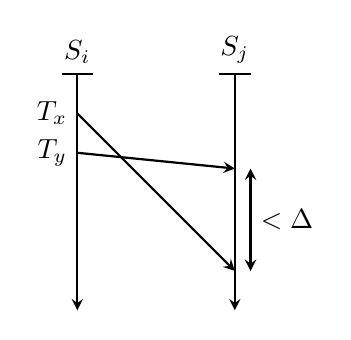
\begin{tikzpicture}[node distance=2cm]
    % s1
    \draw [thick] (1.3,3) -- (1.7,3);
    \draw [thick,<-,>=stealth] (1.5,0) -- (1.5,3) node[anchor=south] {$S_i$};
    % s2
    \draw [thick] (3.3,3) -- (3.7,3);
    \draw [thick,<-,>=stealth] (3.5,0) -- (3.5,3) node[anchor=south] {$S_j$};

    \draw [thick,->,>=stealth] (1.5,2.5) node[left] {$T_x$} -- (3.5,0.5);
    \draw [thick,->,>=stealth] (1.5,2) node[left] {$T_y$} -- (3.5,1.8);

    \draw [thick,<->,>=stealth] (3.7,0.5) -- (3.7,1.8) node[midway,right] {$< \Delta$};

  \end{tikzpicture}
  \caption{An example of the \emph{Delta} protocol preserving reciprocal consistency.}
  \label{delta-abort}
\end{figure}

If $\Delta$ is exceeded all three conflict scenarios can still occur, resulting in half-corrupted edges and the spread of semantic corruption. Figure \ref{corruption-again} displays an example when the \emph{Delta} protocol fails to maintain reciprocal consistency.

\begin{figure}[H]
  \centering
  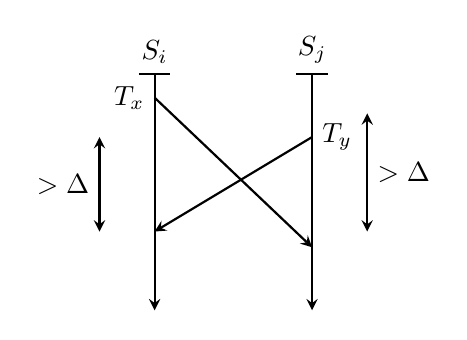
\begin{tikzpicture}[node distance=2cm]
    \draw [thick] (1.3,3) -- (1.7,3);
    \draw [thick,<-,>=stealth] (1.5,0) -- (1.5,3) node[anchor=south] {$S_i$};
    \draw [thick] (3.3,3) -- (3.7,3);
    \draw [thick,<-,>=stealth] (3.5,0) -- (3.5,3) node[anchor=south] {$S_j$};
        \draw [thick,->,>=stealth] (1.5,2.7) node[left] {$T_x$} -- (3.5,0.8);
    \draw [thick,<-,>=stealth] (1.5,1) -- (3.5,2.2)  node[right] {$T_y$};

    \draw [thick,<->,>=stealth] (0.8,1) -- (0.8,2.2) node[midway,left] {$> \Delta$};
    \draw [thick,<->,>=stealth] (4.2,1) -- (4.2,2.5) node[midway,right] {$> \Delta$};
  \end{tikzpicture}
  \caption{An example of the \emph{Delta} protocol failing to preserve reciprocal consistency.}
  \label{corruption-again}
\end{figure}

In summary, the protocol attempts to avoid corruption by aborting transactions but cannot do so in all circumstances. Two questions naturally arise regards the performance of the protocol for different values of  $\Delta$, i) how does the protocol impact on the time until operational corruption? ii) how many transactions are aborted as a result of the protocol?

\section{Modeling}
\label{sec:modeling}

In order to answer i) the model developed in \cite{Ezhilchelvan2018} and fine-tuned in \cite{Webber2019} was extended to measure the impact of the \emph{Delta} protocol\footnote{An empirical evaluation of existing systems was not performed as such an evaluation would have been impractical (need to compare database state at end of experiment with the linearizable truth), slow (real time) and expensive (requiring many hours of storage and compute time)}. A summary of the model is now provided, before discussing the extensions.

Transactions arrive in a Poisson stream with rate $\lambda$ per second. Each transaction contains a random number of read operations, $K$, followed by a single write. Edges in the database are divided into $T$ types, popular edges types have higher access probabilities but are a smaller proportion of the total number of edges, $N$. For each type, a fraction $f$ are distributed edges and the remainder are local edges.

At any moment in time an edge can be in one of four states:
\begin{enumerate}
\item Local and clean.
\item Distributed and clean.
\item Half-corrupted distributed edge arising from interleaved updates.
\item Semantically corrupted.
\end{enumerate}
The valid state transitions are given in Figure \ref{state-transitions}. Note, only distributed edges can be in state 2, but any edge, including local ones, can be in state 3.

\begin{figure}[ht]
  \centering
    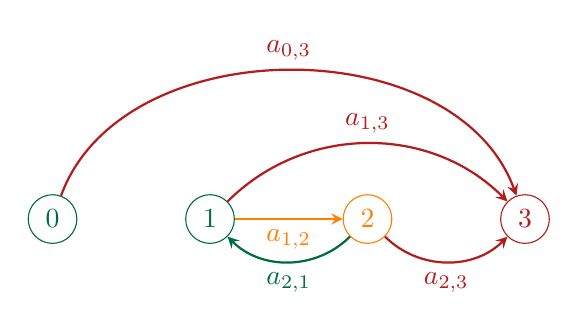
\begin{tikzpicture}[node distance=2cm]
      \node (n0) [circle,draw,radius=0.3, align=center,green] {0};
      \node (n1) [circle,draw,radius=0.3, align=center, right of=n0,green] {1};
      \node (n2) [circle,draw,radius=0.3, align=center, right of=n1,orange] {2};
      \node (n3) [circle,draw,radius=0.3, align=center, right of=n2,red] {3};
      \draw [thick,<-,>=stealth,green] (n1) to[out=-45,in=-135]  node[below] {$a_{2,1}$} (n2);
      \draw [thick,->,>=stealth,orange] (n1)  to[out=0,in=-180] node[below] {$a_{1,2}$} (n2);
      \draw  [thick,->,>=stealth,red] (n2) to[out=-45,in=-135]  node[below] {$a_{2,3}$} (n3);
      \draw  [thick,->,>=stealth,red]  (n0) to[out=70,in=110] node[above] {$a_{0,3}$} (n3);
      \draw  [thick,->,>=stealth,red]  (n1) to[out=45,in=135] node[above] {$a_{1,3}$} (n3);
    \end{tikzpicture}
    \caption{Edge transitions between clean, half-corrupted and semantically corrupt states.}
    \label{state-transitions}
\end{figure}

Probabilities are then derived for a given read operation returning a correct answer (states 1, 2 or the correct record in state 3) and all the reads by a given transaction returning correct answers. Then the probability of edge becoming half-corrupted $q_i$, by a given transaction arriving at time $t$ and operating on edge of type $i$ is derived. These probabilities are used to construct transition rates $a_{i,j}$ between states, which are used to simulate the process of corrupting the database and obtain estimates for the average time to corruption, $U_{\gamma}$. At time $0$, all edges are clean (free from corruption). When a certain fraction, $\gamma$, of all edges become corrupted, the database itself is said to be operationally corrupt.  Note, the model assumes crash-free hardware and bug-free software for simplicity. The reader is directed to \cite{Ezhilchelvan2018} and \cite{Webber2019} for a granular discussion of the initial model.

The \emph{Delta} protocol influences the rate of corruption reducing the probability a transaction corrupts an edge, $q^{new}_i$. To simplify the derivation of the new conflict probability it was assumed that messages sent from the same servers do not arrive out of order, Figure 3(c). This leaves the Figure 6 as the only source of corruption. From this the following probability can be formulated:
$$ q^{new}_i = P \left[ ( T_x >  \Delta + X) \cap (T_y > \Delta-X) \right]$$
The arrival times of $T_x,T_y$ are assumed exponentially distributed , $X \sim \exp (\rho)$, where $\rho = \frac{\lambda P_i}{2N_i}$, the probability of accessing a given end edge of type $i$. The transmission times $M_1, M_2 \sim \exp (\delta)$ and are \emph{iid}. The complete derivation of $q^{new}_i$ is provided in Appendix A.

Of interest, therefore, is: how large or small is the value of $U_\gamma$ for a given value of $\gamma$ under the \emph{Delta} protocol? The answer depends on several parameters characterizing four systemic aspects:
\begin{itemize}
\item \emph{Size and topology of graph database}. Size is expressed by the total number of edges $N$, and the fraction $f$ of edges distributed across servers. We consider a common edge access patterns or topologies: a Scale-free topology, edges have different access probabilities and those that get accessed more frequently tend to be smaller in number.
\item \emph{Workload}. Measured as transactions per second (TPS). Significant for measuring $U_{\gamma}$ are: the fraction of this load that writes after reads and the number of reads that precede a write.
\item \emph{Distributed Write Delays and Choosing $\Delta$}. The smaller the delays the less likely the bound $\Delta$ is violated. Conversely, smaller $\Delta$ is the more likely the bound $\Delta$ is violated.
\end{itemize}

In order to answer (ii), calculating the number of aborts per second for a given $\Delta$ an discrete event-based simulation was constructed. The simulation, focuses on the subset of edges with the highest access probability.


\section{Evaluation}
\label{sec:evaluation}

The model assumes that the distributed graph database  processes many reads-followed-by-write graph queries concurrently, processing both local and distributed edges. The simulation is performed on a Scale-Free graph, such as a social network, human brain, or road network, large enough to make processing non-trivial. There are approximately 7.7 billion local edges, approximately 3.3 million distributed edges (in proportion to good graph partitioning algorithms); a graph of this size would have approximately 1 billion nodes.

The graph consisted of seven edge types, $N_1=10^4, N_2=10^5, N_3=10^6, N_4=10^7,  N_5=10^8, N_6=10^9, N_7=10^10$ with access probabilities $p_1 =0.5, p_2 =0.25, p_3=0.13, p_4=0.06, p_5=0.03, p_6=0.02$ and $p_7 =0.01$. The number of read operations per query is distributed geometrically starting at $2$, with an average of $15$, before a write. In all edge types, a fraction $0.3$ are distributed, the remainder are local. The network delay between servers is exponential distributed with a rate of $200ms$. The database is initial clean and considered to be corrupted when $10$\% ($\gamma = 0.1$) of all edges are corrupted. The time taken until operational corruption $U$, is measured in hours. $U$ considered for a range of transaction arrival rates, $\lambda = (1000, ..., 10000)$; a typical graph workload comprises of 90\% read-only transactions and 10\% read-write transactions \cite{Angles2020}, hence the chosen range reflects the range $\lambda = (10000, ..., 100000)$. We considered 3 values of $\Delta = 1, 5, 10ms$.

\begin{figure}[h]
  \centering
  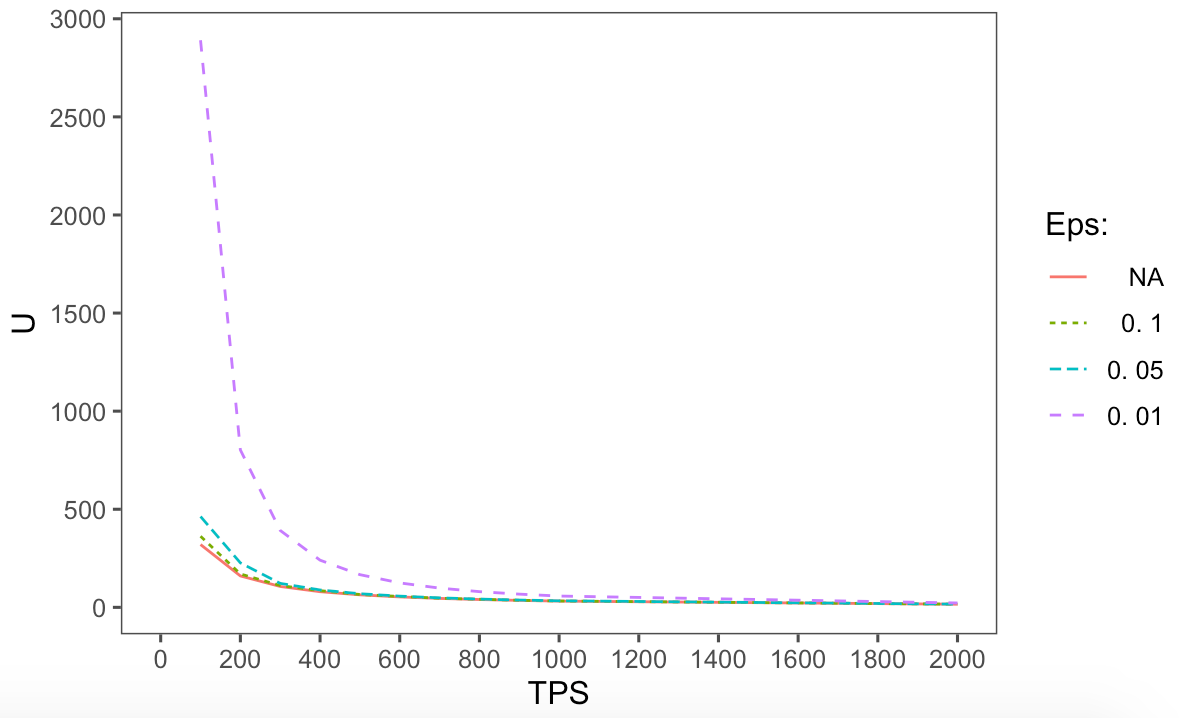
\includegraphics[width=\linewidth]{./images/results}
  \caption{Time until operational corruption under delta protocol}
  \Description{Graph representation.}
  \label{time-to-corruption-results}
\end{figure}

The results for measuring the impact of time until operational corruption are given in Figure \ref{time-to-corruption-results}. %The $\Delta$ has a significant on increasing the time to operational corruption for modest transaction arrival rates ($<1000$).

The abort rates for $\Delta = 1, 5, 10ms$ is given in Figure \ref{aborts-results} for the most popular edge type, $N=10^4$. The simulation was ran for 10 seconds for a range of transaction arrival rates, $\lambda = (1000, ..., 10000)$.


\begin{figure}[h]
  \centering
  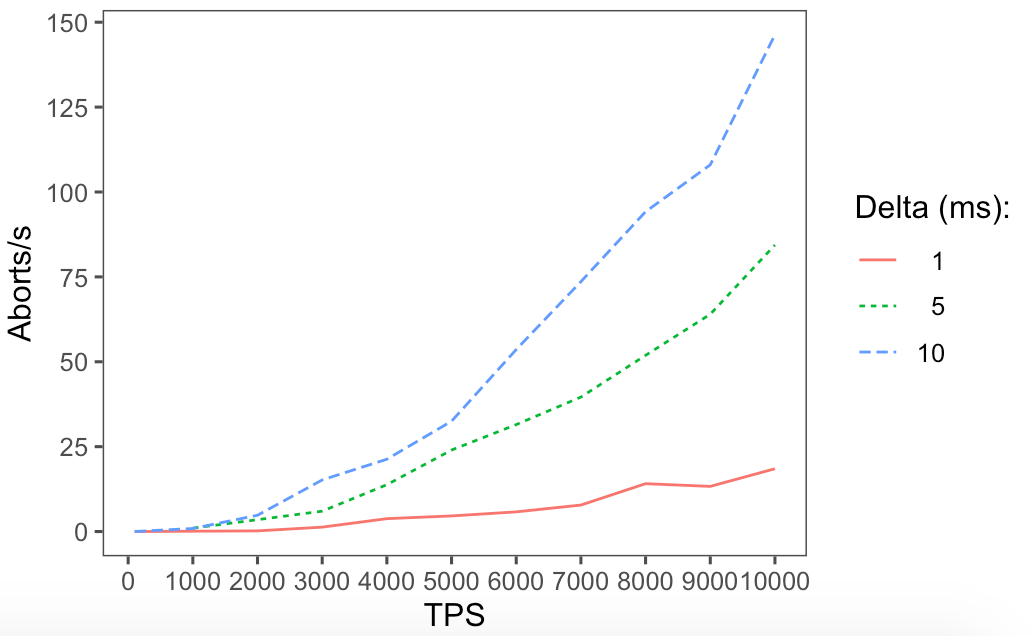
\includegraphics[width=\linewidth]{./images/aborts}
  \caption{Aborts per seconds under protocol}
  \Description{Graph representation.}
  \label{aborts-results}
\end{figure}


\section{Conclusions}

In this paper a lightweight protocol for providing reciprocal consistency and mitigating the problem of high contention in a distributed graph database has been presented. The $\Delta$ protocol leverages the fact writes to edges always consists of two sequential writes. The result is guarantees much weaker than even Read Uncommitted isolation, the weakest ANSI isolation level. However, a mechanism to provide solely reciprocal consistency is believed to be valuable in practice. Concurrency control has been a long researched area, however to the best of our knowledge no other work has presented protocols bespoke to maintaining distributed graph databases.

TODO: More details regards protocol performance.
\section{Acknowledgments}

TODO


\appendix
\section{Appendix}

Figure \ref{corruption-again} presents an interleaving when a distributed edge can become half-corrupted under the \emph{Delta} protocol.

Transaction $T_x$ arrives at $S_i$ at time $t_x$ (let $t=0$) and writes tentatively, with the message delay between servers for $T_x$ to write the edge at $S_j$ being $M_x$. Transaction $T_y$ arrives at $S_j$ at time $t_y$ ($t_y > t_x$) and writes the distributed edge, $T_y$ then takes time $M_y$ to write the edge at $S_i$. If $T_x$ arrives at $S_j$ after $t_y + \Delta$ and $T_y$ arrives at $S_i$ after $t_x + \Delta$ the edge can become half-corrupted. Letting $t_x = 0 $, the probability that $T_x$ and $T_y$ conflict can be formulated as: $$ P \left[ ( T_x >  \Delta + X) \cap (T_y > \Delta-X) \right]$$.

The arrival times of $T_x,T_y$ are assumed exponentially distributed , $T \sim \exp (\rho)$. Where, $ \rho  = \frac{\lambda P_i}{2N_i}$, the probability a given operation accesses the incorrect record of a half-corrupted edge of type $i$. The transmission times between servers $M_1, M_2 \sim \exp (\delta)$ and are \emph{iid}.

% Therefore,  $$ g(y) = \delta e^{-\delta y} $$

Therefore,
\begin{dmath*}
  q^{new}_{i} =  {P \left[ ( T_1 >  d + X) \cap (T_2 > d-X)  \right]} \\
  =  \int_{0}^{d}  \frac{\lambda P_i}{2 N_i} e^{-\frac{\lambda P_i}{2 N_i} x} e^{-\delta (d+x)} e^{-\delta (d-x)} dx + \int_{d}^{\infty} \frac{\lambda P_i}{2 N_i} e^{-\frac{\lambda P_i}{2 N_i} x} e^{-\delta (d+x)} dx  \\
  =  e^{-2 d \delta} - \left( \frac{\delta}{\frac{\lambda P_i}{2 N_i} + \delta} \right) e^{-(\frac{\lambda P_i}{2 N_i}+ 2\delta)d} \\
\end{dmath*}

% To choose to bound $\Delta$ consider the probability of the message delay exceeding  $\Delta$.
% \begin{align*}
%   P \left[ M > \Delta \right] & = 1 - e^{- \delta \Delta} \\
%   1 - e^{- \delta \Delta} & = 1 - \epsilon \\
%   e^{- \delta d} & = \epsilon  \\
%   \Delta & = - \frac{\ln(\epsilon)}{\delta}
% \end{align*}

% Substituting $\Delta$ into the above equation yields the conflict probability for a given $\epsilon$. For example, $ e = 0.001$ gives a $0.001$ \% probability the message delay exceeds $\Delta$, for this  $\Delta = 0.035s$
% \begin{align}
%   e^{- \lambda d} =  e^{-\delta d \frac{\lambda}{\delta}} = \epsilon^{\frac{\lambda}{\delta}} \label{eqn7}
% \end{align}
% Therefore, from (\ref{eqn5} and  (\ref{eqn7}),
% \begin{align}
%   & = \epsilon^2 - \frac{\delta}{\frac{\lambda P_i}{2 N_i} + \delta} e^{-\frac{\lambda P_i}{2 N_i} d} \epsilon^2 \\
%   & = \epsilon^2 \left[1 -\frac{\delta}{\frac{\lambda P_i}{2 N_i} + \delta} e^{-\frac{\lambda P_i}{2 N_i} d} \right]
% \end{align}


%Where, $ E \left[ T_1 \right] = E \left[ T_2\right] = \frac{1}{\delta}$.
%Therefore, $$ f(x) =\frac{\lambda P_i}{2N_i} e^{-\frac{\lambda P_i}{2N_i} x} $$

%  =   \int_{0}^{d}  \frac{\lambda P_i}{2 N_i} e^{-\frac{\lambda P_i}{2 N_i} x} e^{-\delta 2 d} dx +  \int_{d}^{\infty} \frac{\lambda P_i}{2 N_i} e^{-\delta d} e^{-(\frac{\lambda P_i}{2 N_i} + \delta)x}  dx  \\
%         =   e^{-2 d \delta} \left[1 - e^{-\frac{\lambda P_i}{2 N_i} d} \right] + \frac{\frac{\lambda P_i}{2 N_i} e^{-\delta d}}{\frac{\lambda P_i}{2 N_i} + \delta} e^{-(\frac{\lambda P_i}{2 N_i} + \delta)d} \\







\bibliographystyle{ACM-Reference-Format}
\bibliography{papoc}

\end{document}
\endinput
